\documentclass[11pt]{article}
\usepackage[utf8]{inputenc}
\usepackage[T1]{fontenc}
\usepackage{amsmath}
\usepackage{amssymb}
\usepackage{multicol}
\usepackage{geometry}
\usepackage{tikz}
\usepackage{enumitem}
\usepackage{xcolor}
\usepackage{titlesec}

% Configurações de layout
\geometry{a4paper, left=1cm, right=1cm, top=0.5cm, bottom=1.2cm}
\setlength{\columnseprule}{0.4pt}

% Cores para títulos
\titleformat{\section}{\normalfont\Large\bfseries\color{blue}}{\thesection}{1em}{}
\titleformat{\subsection}{\normalfont\large\bfseries\color{red}}{\thesubsection}{1em}{}

\title{\textcolor{red}{Primeiro Trimestre: Matemática Financeira
    \\Juros Simples}}
\author{Professor: Jefferson}
\date{}

\begin{document}

\maketitle
\vspace{-1cm}

%\begin{center}
%\large{Nome: \underline{\hspace{8cm}} \quad Turma: \underline{\hspace{3cm}}}
%\end{center}

\begin{multicols}{2}

\section*{Instruções}
    \textbf{Copie e responda no caderno.}

\section*{Conceitos Básicos}

\subsection*{Capital (C)}
Valor inicial aplicado ou emprestado.

\subsection*{Taxa de Juros (i)}
Porcentagem cobrada pelo empréstimo ou ganha pelo investimento.

\subsection*{Tempo (t)}
Período da aplicação (em meses, anos, etc.).

\subsection*{Montante (M)}
Valor total ao final do período:
\[
M = C + J
\]
onde $J$ são os juros.

\section*{Juros Simples - Fórmula Principal}


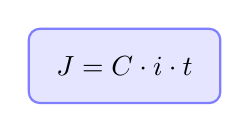
\begin{tikzpicture}
\node[rectangle, fill=blue!10, rounded corners, inner sep=10pt, draw=blue!50, thick] (box) {
$\displaystyle J = C \cdot i \cdot t$
};
\end{tikzpicture}

\subsection*{Fórmulas Derivadas}
\begin{itemize}
\item Juros: $J = C \cdot i \cdot t$
\item Montante: $M = C \cdot (1 + i \cdot t)$
\item Capital: $C = \dfrac{M}{1 + i \cdot t}$
\item Taxa: $i = \dfrac{J}{C \cdot t}$
\item Tempo: $t = \dfrac{J}{C \cdot i}$
\end{itemize}

\subsection*{Características Fundamentais}
\begin{itemize}
\item \textbf{Crescimento linear} (progressão aritmética)
\item Juros constantes em todos os períodos
\item Calculado sempre sobre o capital inicial
\item O juro não é incorporado ao capital
\item Ideal para períodos curtos
\end{itemize}

\section*{Representação Gráfica}

\begin{center}
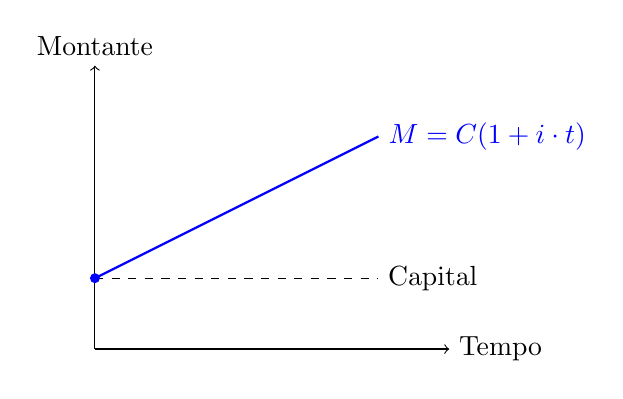
\begin{tikzpicture}[scale=0.9]
\draw[->] (0,0) -- (5,0) node[right] {Tempo};
\draw[->] (0,0) -- (0,4) node[above] {Montante};
\draw[blue, thick, domain=0:4] plot (\x, {1 + 0.5*\x}) node[right] {$M = C(1 + i\cdot t)$};
\draw[dashed] (0,1) -- (4,1) node[right] {Capital};
\fill[blue] (0,1) circle (2pt);
\end{tikzpicture}
\end{center}

A função do montante é uma reta crescente com inclinação $C \cdot i$.

\section*{Exercícios Básicos - Juros Simples}

\begin{enumerate}[leftmargin=*]

\item Calcule os juros simples:
\begin{enumerate}[label=\alph*)]
\item $C = R\$ 1000$, $i = 2\%$ a.m., $t = 6$ meses
\item $C = R\$ 500$, $i = 1,5\%$ a.m., $t = 1$ ano
\item $C = R\$ 2000$, $i = 10\%$ a.a., $t = 2$ anos
\end{enumerate}

\item Calcule o montante a juros simples:
\begin{enumerate}[label=\alph*)]
\item $C = R\$ 800$, $i = 3\%$ a.m., $t = 5$ meses
\item $C = R\$ 1500$, $i = 2\%$ a.m., $t = 8$ meses
\item $C = R\$ 3000$, $i = 15\%$ a.a., $t = 3$ anos
\end{enumerate}

\item Complete a tabela (juros simples):
\begin{center}
\begin{tabular}{|c|c|c|c|}
\hline
\textbf{C} & \textbf{i} & \textbf{t} & \textbf{J} \\
\hline
R\$ 1000 & 2\% a.m. & 6 meses & \\
\hline
R\$ 500 & 12\% a.a. & 2 anos & \\
\hline
R\$ 2000 & 1,5\% a.m. & 1 ano & \\
\hline
\end{tabular}
\end{center}

\item Problemas práticos:
\begin{enumerate}[label=\alph*)]
\item João aplicou R\$ 800 a juros simples de 3\% a.m. por 5 meses. Qual o montante?
\item Um capital de R\$ 1200 rendeu R\$ 288 em 1 ano. Qual a taxa anual?
\item Qual o tempo necessário para R\$ 2000 render R\$ 600 a 5\% a.m.?
\end{enumerate}

\end{enumerate}

\section*{Conversão de Taxas - Juros Simples}

\subsection*{Taxas Proporcionais}
Em juros simples, taxas são proporcionais ao tempo:

\[
i_{\text{anual}} = 12 \cdot i_{\text{mensal}}
\]
\[
i_{\text{mensal}} = \frac{i_{\text{anual}}}{12}
\]
\[
i_{\text{diária}} = \frac{i_{\text{mensal}}}{30}
\]

\subsection*{Exemplos:}
\begin{itemize}
\item 2\% a.m. = 24\% a.a.
\item 18\% a.a. = 1,5\% a.m.
\item 0,1\% a.d. = 3\% a.m.
\end{itemize}

\section*{Exercícios Intermediários}

\begin{enumerate}[leftmargin=*, start=5]

\item Calcule a taxa mensal equivalente a:
\begin{enumerate}[label=\alph*)]
\item 12\% a.a.
\item 24\% a.a.
\item 30\% a.a.
\end{enumerate}

\item Um capital de R\$ 2000 foi aplicado a juros simples:
\begin{enumerate}[label=\alph*)]
\item Rendendo R\$ 600 em 1 ano. Qual a taxa anual?
\item Rendendo R\$ 450 em 9 meses. Qual a taxa mensal?
\item Qual o montante após 2 anos à taxa de 8\% a.a.?
\end{enumerate}

\item Determine o tempo necessário:
\begin{enumerate}[label=\alph*)]
\item Duplicar um capital a 10\% a.a.
\item Triplicar um capital a 5\% a.m.
\item R\$ 1500 render R\$ 600 a 2\% a.m.
\end{enumerate}

\item Problemas contextualizados:
\begin{enumerate}[label=\alph*)]
\item Empréstimo de R\$ 5000 a 2\% a.m. por 10 meses. Qual o total a pagar?
\item Uma aplicação de R\$ 3000 rendeu R\$ 450 em 6 meses. Qual a taxa mensal?
\item Quantos meses são necessários para R\$ 2000 virar R\$ 2600 a 1,5\% a.m.?
\end{enumerate}

\item Análise de gráfico:
\begin{center}
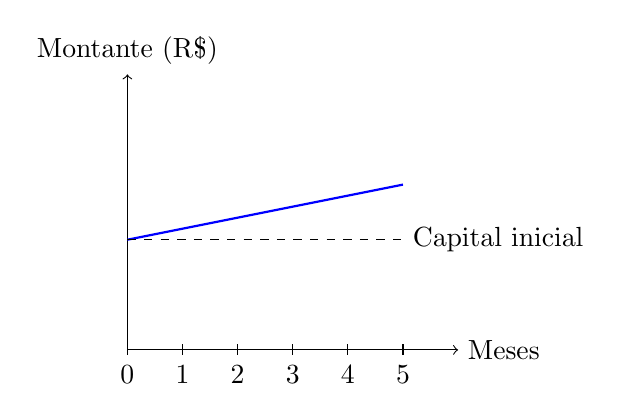
\begin{tikzpicture}[scale=0.7]
\draw[->] (0,0) -- (6,0) node[right] {Meses};
\draw[->] (0,0) -- (0,5) node[above] {Montante (R\$)};
\draw[blue, thick] (0,2) -- (1,2.2) -- (2,2.4) -- (3,2.6) -- (4,2.8) -- (5,3.0);
\foreach \x in {0,1,2,3,4,5} \draw (\x,0.1) -- (\x,-0.1) node[below] {\x};
\draw[dashed] (0,2) -- (5,2) node[right] {Capital inicial};
\end{tikzpicture}
\end{center}
\begin{enumerate}[label=\alph*)]
\item Qual o capital inicial?
\item Qual a taxa mensal?
\item Qual o montante após 8 meses?
\end{enumerate}

\end{enumerate}

\section*{Problemas Avançados}

\begin{enumerate}[leftmargin=*, start=9]

\item Regras práticas:
\begin{enumerate}[label=\alph*)]
\item Um capital aplicado a juros simples dobra em 10 anos. Qual a taxa?
\item Em quanto tempo um capital quadruplica a 5\% a.m.?
\item Qual capital rende R\$ 1000 em 8 meses a 2,5\% a.m.?
\end{enumerate}

\item Comparação de propostas:
\begin{enumerate}[label=\alph*)]
\item Banco A: R\$ 5000, 2,2\% a.m., 12 meses
\item Banco B: R\$ 5000, 2,5\% a.m., 10 meses
\item Qual cobra menos juros?
\end{enumerate}

\item Problema de lógica:
\begin{enumerate}[label=\alph*)]
\item Um capital aplicado a juros simples duplica em 8 anos.
  Em quanto tempo triplicaria?
\item Se R\$ 4000 rende R\$ 1000 em 5 meses, qual a taxa anual?
\end{enumerate}

\item Desafio final:
\begin{enumerate}[label=\alph*)]
\item Determine a fórmula do montante para depósitos mensais iguais de R\$ 100 a juros simples de 1\% a.m. após 12 meses.
\item Compare: R\$ 1000 a 2\% a.m. por 2 anos (simples) vs R\$ 1000 a 1,8\% a.m. por 2 anos (simples)
\end{enumerate}

\end{enumerate}

\section*{Dicas Importantes}

\begin{itemize}
\item \textbf{Sempre} verifique se taxa e tempo estão na mesma unidade
\item \textbf{Converta} taxas proporcionais quando necessário
\item \textbf{Juros simples} = crescimento linear
\item \textbf{Para períodos fracionários}, a fórmula é a mesma
\item \textbf{Cuidado} com meses de 30 ou 31 dias (use mês comercial = 30 dias)
\end{itemize}

\end{multicols}

\end{document}
